%%%%%%%%%%%%%%%%%%%%%%%%%%%%%%%%%%%%%%%%%%%%%%%%%%%%%%%%%%%%%%%%%
% Contents : The third parties chapter
% $Id : grisbi-manuel-third.tex, v 0.4 2002/10/27 Daniel Cartron
% $Id : grisbi-manuel-third.tex, v 0.5.0 2004/06/01 Loic Breilloux
% some of its content was in tips chapter : 
% $Id : grisbi-manuel-tips.tex, v 0.4 2002/10/27 Daniel Cartron
% $Id : grisbi-manuel-third.tex, v 0.6.0 2011/11/17 Jean-Luc Duflot
% some of its content was in tips chapter :
% $Id : grisbi-manuel-tips.tex, v 0.5.0 2004/06/01 Loic Breilloux
% $Id : grisbi-manuel-third.tex, v 0.8.9 2012/04/27 Jean-Luc Duflot
% $Id : grisbi-manuel-third.tex, v 1.0 2014/02/12 Jean-Luc Duflot
%%%%%%%%%%%%%%%%%%%%%%%%%%%%%%%%%%%%%%%%%%%%%%%%%%%%%%%%%%%%%%%%%

\chapter{Tiers\label{thirdparties}}


On appelle tiers la personne ou plus généralement l'organisation avec qui on a
une relation financière, par exemple un ami, un commerçant ou une administration.  Ne pas confondre avec la catégorie, qui définit  la nature de cette relation, par exemple \og Loisirs \fg{} ou \og Habillement \fg{}. D'une autre manière, \emph{qui} et \emph{quoi}\ldots

Bien sûr, si vous changez de fournisseur sans cesse, vous pouvez créer un tiers fournisseur générique (ex : \emph{Station-service}) mais votre comptabilité sera moins précise.

Outre ces tiers, peuvent aussi exister ceux que l'on pourrait appeler des 
\indexword{\emph{tiers financiers}}\index{tiers !financiers}. En effet, lorsque vous faites un virement de compte à compte, il est intéressant de créer un tiers spécifique pour ce genre d'opération, par exemple 
\emph{Alimentation des comptes d'épargne}, ou bien \emph{Remise de chèques}, ou encore \emph{Régularisation d'avances}. Ceci vous permettra ultérieurement une analyse plus fine de vos finances. 

% espace pour changement de thème
\vspacepdf{5mm}
L'onglet \menu{Tiers} sert à gérer tous les tiers de votre fichier de comptes.

%espace pour changement de thème
\vspacepdf{5mm}
Pour avoir accès à la gestion des tiers, cliquez sur \menu{Tiers} dans le panneau de navigation, ou sélectionnez \menu{Tiers} avec la barre d'information (voir le chapitre \vref{home}, \menu{Accueil}).

%espace pour changement de thème
\vspacepdf{5mm}
La barre d'information affiche, à gauche, le nom du tiers sélectionné dans le pavé des détails et, complètement à droite, le solde des opérations affectées.

%espace pour changement de thème
\vspacepdf{5mm}
Le pavé des détails affiche deux éléments :
\begin{itemize}
	 \item la barre d'outils ;
	 \item la liste des tiers.
\end{itemize}


\section{Barre d'outils\label{thirdparties-functions}}


La barre d'outils des tiers présente les fonctions suivantes  :

\begin{itemize}
	 \item \menu{Nouveau tiers} : ouvre une fenêtre pour créer un nouveau tiers ;
	 \item \menu{Supprimer} : supprime le tiers sélectionné ;
	 \item \menu{Éditer} : ouvre une fenêtre pour modifier le nom ou la description du tiers sélectionné ;
	 \item \menu{Affichage} : ouvre un menu déroulant pour afficher soit la \menu{Vue des tiers uniquement}, soit la \menu{Vue complète}, pour tous les tiers avec leurs opérations, ainsi que le choix d'\menu{Afficher les tiers inutilisés} ;
	 \item \menu{Gérer les tiers} : ouvre l'assistant de gestion des tiers ;
	 \item \menu{Supprimer les tiers inutilisés} : permet de supprimer les tiers n'ayant aucune opération.
\end{itemize}

%espace pour changement de thème
\vspacepdf{5mm}
La barre d'outils peut être déplacée dans l'écran en cliquant sur sa poignée (petit rectangle vertical à gauche de la barre) et en la déplaçant. Pour la réattacher à son emplacement d'origine dans le pavé des détails, la remettre en haut de la fenêtre, le haut de la poignée placé sur le petit trait qui visualise sa place d'origine.


\section{Liste des tiers\label{thirdparties-list}}


La liste des tiers s'affiche dans le panneau des \ifIllustration détails\refimage{thirdparties-list-img}.
\else détails.
\fi
% image centrée
\ifIllustration
\begin{figure}[htbp]
\begin{center}
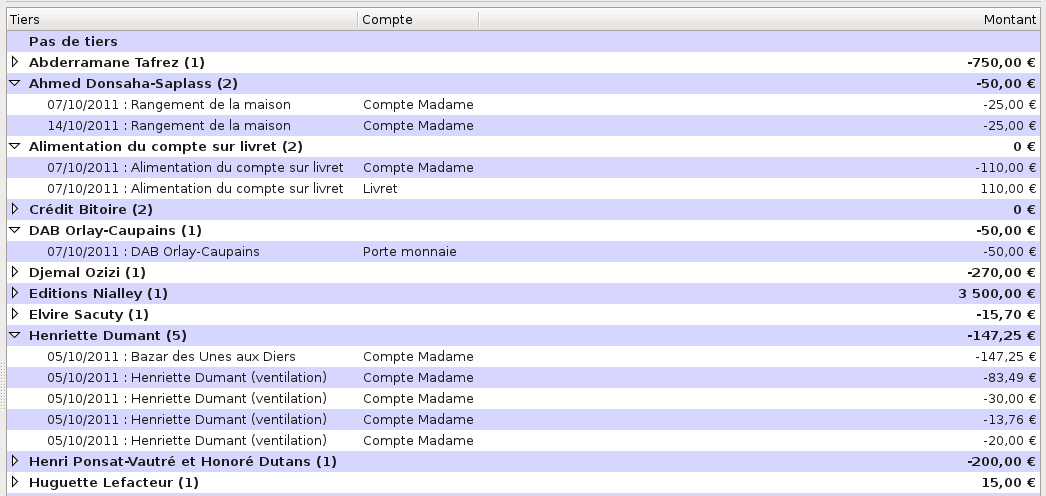
\includegraphics[scale=0.5]{image/screenshot/thirdparties_list}
\end{center}
\caption{Liste des tiers}
\label{thirdparties-list-img}
\end{figure}
% image centrée
\fi

Elle affiche en haut la barre des libellés des colonnes ; ses champs d'affichage sont les suivants :
\begin{itemize}
	 \item le nom du tiers ;
	 \item le compte concerné ;
	 \item le montant total des opérations affectées à ce tiers, et le montant de chaque opération si la ligne du tiers est déroulée.
\end{itemize}

%espace pour changement de thème
\vspacepdf{5mm}
Vous pouvez déplacer la liste des tiers vers le haut ou vers le bas avec la molette de la souris, ou bien avec la souris et l'ascenseur vertical. Le déplacement éventuel vers la gauche ou la droite se fait avec la souris et l'ascenseur horizontal.

%espace pour changement de thème
\vspacepdf{5mm}
La liste des tiers affiche tous les tiers de votre fichier de comptes par ordre alphabétique, avec une seule exception : le premier tiers affiché est toujours le tiers de libellé \indexword{\menu{Pas de tiers}}\index{tiers !pas de tiers}, qui reçoit toutes les opérations dont le tiers n'est pas défini.


Le nombre d'opérations affectées à chaque tiers s'affiche, entre parenthèses, à la suite de son nom, et le montant total des opérations affectées à ces tiers s'affiche dans la colonne \menu{Montant}, à droite sur la même ligne.

% Bogue connu  : en cliquant sur une ligne de tiers, la barre d'information devrait afficher le total, mais n'affiche que 0. 

% espace avant Attention ou Note  : 5 mm
\vspacepdf{5mm}
\textbf{Note} : vous pouvez configurer la \indexword{devise des totaux}\index{devise !totaux} de tous les tiers dans le menu \menu{Édition - Préférences} (voir le paragraphe \vref{setup-display-third-currencies}, \menu{Devises des totaux}).

\ifIllustration
% saut de page pour titre solidaire
\newpage
\fi


\section{Sélection d'un tiers\label{thirdparties-selection}}


Pour sélectionner un tiers, vous avez deux moyens :

\begin{itemize}
	 \item cliquez sur sa ligne ;
	 \item déplacez la sélection avec les touches du clavier \key{Flèche Haut}, \key{Flèche Bas}, \key{Page Haut} ou \key{Page Bas}.
\end{itemize}

Le nom du tiers apparaît alors sur fond rose{\couleur}.


\section{Les opérations d'un tiers\label{thirdparties-transactions}}


Pour \indexword{afficher} les opérations affectées à un tiers\index{affichage !tiers}, cliquez sur le petit triangle à gauche de son nom, ou bien double-cliquez sur sa ligne,
% ou bien sélectionnez-le et appuyez sur la barre d'espace (non fonctionnel) 
ce qui déroule la liste. Les opérations sont alors décrites sur une seule ligne, avec leur date, leur remarque éventuelle, le nom du compte concerné et leur montant.
%le seul moyen de dérouler la liste est de cliquer sur le petit triangle. il devrait y avoir un moyen avec le clavier, comme ça existe avec le formulaire de saisie, où l'on peut utiliser la barre d'espace pour le moyen de paiement, ou la touche flèche bas pour la catégorie..

\textbf{Note} : ces triangles peuvent être remplacés, en fonction du thème de l'environnement de bureau ou du gestionnaire de fenêtres que vous utilisez, par d'autres caractères tels que +, -, >, <, etc.

% espace après Attention ou Note  : 5 mm
\vspacepdf{5mm}

Vous pouvez afficher plusieurs \indexword{tiers déroulés}\index{tiers !déroulés}. Pour ne plus les afficher, \indexword{enroulez les tiers}\index{tiers !enroulés} en cliquant sur le petit triangle à gauche de leur nom, ou bien double-cliquez sur leur ligne. Vous pouvez aussi dérouler ou enrouler tous les tiers de la liste, en cliquant sur l'outil \menu{Affichage}\index{affichage !tiers} dans la barre d'outils et en choisissant \menu{Vue complète}. Pour afficher seulement les tiers, cliquez sur l'outil \menu{Affichage} dans la barre d'outils et choisissez \menu{Vue des tiers uniquement}.

%espace pour changement de thème
\vspacepdf{5mm}
Vous pouvez \indexword{déplacer une opération d'un tiers}\index{tiers !déplacement d'opération} vers un autre tiers de la liste (sauf vers \indexword{\menu{Pas de tiers}}\index{tiers !pas de tiers}), en sélectionnant cette opération et en faisant un glisser-déplacer sur le tiers cible, exactement à l'endroit où son nom est entouré d'une bordure pointillée.

%espace pour changement de thème
\vspacepdf{5mm}
Un \indexword{double-clic sur une ligne d'opération} d'un tiers\index{tiers !double-clic} ferme l'onglet \menu{Tiers}, ouvre l'onglet \menu{Comptes} et le sous-onglet du compte contenant cette opération, sélectionne l'opération concernée et l'affiche dans le formulaire de saisie. De cette façon, cette opération peut être modifiée facilement.


\section{Création d'un tiers\label{thirdparties-new}}


\ifIllustration
% image entourée par un paragraphe ( picins)
% Pas de référence à l'illustration car erreur de numéro de figure avec picins.
% supprimé car en html les figures entourées ne sont pas numérotées, et la numérotation des figures centrées décalée par rapport au pdf
%\piccaption{Création d'un tiers}
\label{thirdparties-new-img}
\parpic[r]{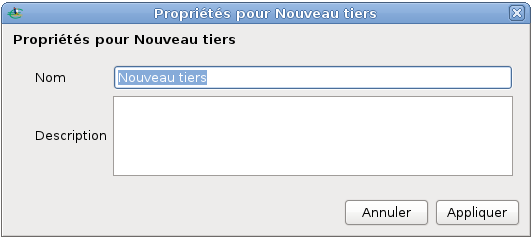
\includegraphics[scale=0.5]{image/screenshot/thirdparties_new}}
% image entourée par un paragraphe ( picins)
\fi

\noindent La façon la plus immédiate pour créer un tiers est de saisir son nom au cours de la saisie d'une nouvelle opération dans l'onglet des comptes (voir la section \vref{transactions-fillcombo}, \menu{Nouveau tiers, catégorie ou imputation budgétaire}) ; mais vous pouvez aussi créer un tiers ici, en cliquant sur l'outil \menu{Nouveau tiers}. Une boîte de dialogue s'ouvre ; renseignez le nom du tiers, et éventuellement une description, puis validez : il apparaît dans la liste des tiers, mais c'est encore un tiers inutilisé, puisqu'aucune opération ne lui est encore affectée (voir la section \vref{thirdparties-unused}, \menu{Tiers inutilisés}).

% espace avant Attention ou Note  : 5 mm
\vspacepdf{5mm}
\textbf{Note} : il n'est pas prévu d'affichage de plus d'informations pour les tiers, par exemple plusieurs champs pour l'adresse, le téléphone, etc. En effet, il nous semble plus intéressant de prévoir dans le futur une liaison avec un gestionnaire de carnet d'adresses de \gls{Gnome} ou de \gls{KDE}, ce qui permettra une gestion beaucoup plus poussée des tiers.

% espace avant Attention ou Note  : 5 mm
\vspacepdf{5mm}
\textbf{Note} : dans tous les cas, un tiers, même inutilisé, s'affiche dans la liste déroulante du formulaire de saisie d'opération, ce qui permet de le sélectionner.


\section{Modification d'un tiers\label{thirdparties-modify}}


Pour modifier un tiers, procédez comme suit :
% espace avant image 5mm
\vspacepdf{3mm}

\begin{enumerate}
	\ifIllustration
	% image entourée par une liste (picins)
	% Pas de référence à l'illustration car erreur de numéro de figure avec picins.
	% supprimé car en html les figures entourées ne sont pas numérotées, et la numérotation des figures centrées décalée par rapport au pdf
	%\piccaption{Propriétés d'un tiers}
	\label{thirdparties-infos-img}
	\parpic[r]{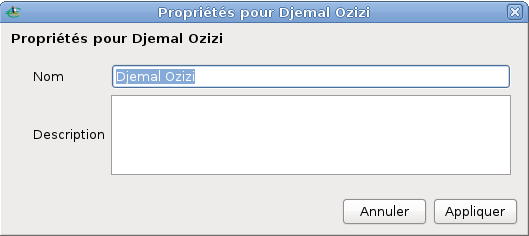
\includegraphics[scale=0.51]{image/screenshot/thirdparties_infos}}
	% image entourée par une liste (picins)	
	\fi
	 \item sélectionnez-le dans la liste ;
	 \item cliquez sur l'outil \menu{Éditer} dans la barre d'outils ;
	 \item une boîte de dialogue s'ouvre : vous pouvez y modifier son nom et sa  description ;
	 \item validez.
\end{enumerate}

\ifIllustration
% espace après légende 10mm
\vspacepdf{5mm}
\fi

\ifIllustration
% espace après image entourée
\vspacehevea{16mm}
\fi


\section{Gestion des tiers\label{thirdparties-management}}


La gestion des tiers permet de modifier le nom de plusieurs tiers à la fois. La méthode consiste à remplacer une chaîne de caractères par une autre en utilisant le \indexword{caractère générique}\index{caractère générique  !\%}  \og  \%  \fg{}, qui remplace tout autre caractère.

Pour gérer les tiers, cliquez sur l'outil \menu{Gérer les tiers} dans la barre d'outils. L'assistant de gestion des tiers s'ouvre, qui comprend quatre étapes ; suivez les instructions données à chaque étape :
\begin{enumerate}
	 \item un avertissement de précautions à prendre avant de continuer ;
	 \item le choix de la \indexword{chaîne de caractères}\index{chaîne de caractères} à remplacer (\menu{Choisir un tiers}) et de celle de remplacement (\menu{Entrez le nouveau tiers}) ; de plus deux options vous sont proposées :
		\begin{itemize}
			 \item \menu{Extraire un numéro à enregistrer dans \No chèque/virement} : si l'ancien tiers contient un numéro qui peut être assimilé à celui d'un chèque ou d'un virement, Grisbi le déplacera dans le champ \og \No chèque/virement \fg{}, mais le numéro de chèque/virement éventuellement déjà présent sera supprimé,
			\item \menu{Sauvegarder les tiers dans les remarques} : tous les tiers seront écrits dans le champ \menu{Remarques}, et les remarques éventuellement déjà présentes seront supprimées ;
			
			\strong{Attention} : si vous cochez ces options, les données existantes (\No chèque ou Remarques) seront remplacées par les nouvelles données (\No intégré dans le nom du tiers ou nom du tiers).
			% espace après Attention ou Note  : 5 mm
			%\vspacepdf{5mm}
		\end{itemize}
	 \item le bilan des remplacements qui vont être effectués ; vous pouvez y 	sélectionner ou désélectionner les remplacements que Grisbi a trouvé à faire selon les critères définis à l'étape précédente ;
	 \item la validation finale.
\end{enumerate}

\ifIllustration
% saut de page pour paragraphe solidaire
\newpage
\fi


\section{Suppression d'un tiers\label{thirdparties-delete}}


Pour supprimer un tiers, procédez comme suit :

\begin{enumerate}
	\ifIllustration
	% image entourée par une liste (picins)
	% Pas de référence à l'illustration car erreur de numéro de figure avec picins.
	\pichskip{7mm}
	% supprimé car en html les figures entourées ne sont pas numérotées, et la numérotation des figures centrées décalée par rapport au pdf
	%\piccaption{Suppression d'un tiers}
	\label{thirdparties-delete-img}
	\parpic[r]{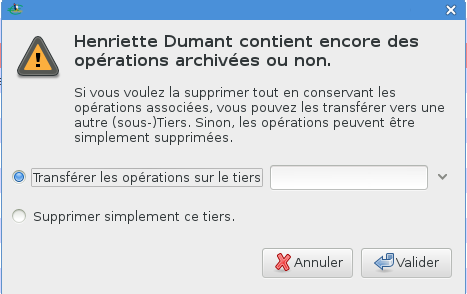
\includegraphics[scale=0.51]{image/screenshot/thirdparties_delete}}
	% image entourée par une liste (picins)	
	\fi
	 \item sélectionnez-le dans la liste ;
	 \item cliquez sur l'outil \menu{Supprimer} dans la barre d'outils ;
	 \item une  boîte de dialogue s'ouvre et vous propose soit de transférer les opérations de ce tiers vers un autre tiers que vous choisissez dans la liste déroulante, soit de le supprimer purement et simplement, \emph{y compris toutes ses opérations} ;
	 \item faites votre choix puis validez.
\end{enumerate}

\ifIllustration
% espace après légende 10mm
\vspacepdf{5mm}
\fi
 
\strong{Attention} : la suppression d'un tiers est \indexword{irréversible}\index{opération !irréversible} !

% espace avant Attention ou Note  : 5 mm
\vspacepdf{5mm}
\textbf{Note} : si le tiers que vous voulez supprimer ne contient aucune opération, aucune boîte de dialogue ne s'ouvrira et Grisbi le supprimera immédiatement.

\ifIllustration
% espace après image entourée
\vspacehevea{2mm}
\fi


\section{Tiers inutilisés\label{thirdparties-unused}}

Un tiers inutilisé est un tiers auquel n'est affectée aucune opération. C'est le cas d'un nouveau tiers quand vous venez juste de le créer avec l'outil \menu{Nouveau tiers}, soit d'un ancien tiers dont toutes les opérations ont été supprimées ou réaffectées vers d'autres tiers.

% espace avant Attention ou Note  : 5 mm
\vspacepdf{5mm}
\textbf{Note} : si vous fermez et réouvrez Grisbi après la création d'un nouveau tiers, il ne sera plus affiché dans la liste des tiers, car il ne contient pas encore d'opération : cela évite l'affichage des tiers inutilisés, qui allonge la liste des tiers souvent très longue ; mais ce tiers apparaîtra dans la liste dès qu'une opération lui aura été affectée.

%espace pour changement de thème
\vspacepdf{5mm}
Pour \indexword{afficher les tiers inutilisés}\index{tiers inutilisés !affichage}\index{affichage !tiers inutilisés}, sélectionnez \menu{Afficher les tiers inutilisés} dans l'outil \menu{Affichage}, qui affiche aussi le nombre de ces tiers.

% espace avant Attention ou Note  : 5 mm
\vspacepdf{5mm}
\textbf{Note} : dans tous les cas, un tiers, même inutilisé, s'affiche dans la liste déroulante du formulaire de saisie d'opération, ce qui permet de le sélectionner.

%espace pour changement de thème
\vspacepdf{5mm}
Pour \indexword{supprimer tous les tiers inutilisés}\index{tiers inutilisés !supprimer}, cliquez sur l'outil \menu{Supprimer les tiers inutilisés} dans la barre d'outils. Une  boîte de dialogue s'ouvre et vous demande la confirmation de cette action. Si vous la validez, une autre boîte affiche le nombre de tiers supprimés.

% espace avant Attention ou Note  : 5 mm
\vspacepdf{5mm}
\strong{Attention} : la suppression des tiers inutilisés est \indexword{irréversible}\index{opération !irréversible} !

\ifIllustration
% saut de page pour titre solidaire
\newpage
\fi


\section{Tiers virtuels\label{thirdparties-virtualCreate}}


Grisbi vous permet d'utiliser des \indexword{tiers virtuels}\index{tiers virtuel} : un tiers virtuel est un \emph{état} qui représente une liste de plusieurs tiers.

Lorsque vous saisissez une opération avec pour tiers un tiers virtuel, Grisbi enregistre, au moment de sa validation, une opération identique (montant, catégorie, imputation budgétaire, moyen de paiement etc.) pour \emph{chacun} des tiers représentés par ce tiers virtuel. Par exemple, vous pouvez saisir en une seule fois un appel à cotisation pour 200 adhérents d'une association, ce qui représente un gain de temps très appréciable \ldots

%espace pour changement de thème
\vspacepdf{5mm}
Pour créer un tiers virtuel, créez un état contenant une liste de tiers : voir le paragraphe \vref{reportscreation-display-general-virtualThird}, \menu{Tiers virtuel}.

% espace avant Attention ou Note  : 5 mm
\vspacepdf{5mm}
\textbf{Note} : comme un tiers virtuel est un état, il ne s'affiche pas dans la liste des tiers, mais dans celle des états, et il est géré de la même manière que les autres états. 

%espace pour changement de thème
\vspacepdf{5mm}
Pour modifier un tiers virtuel, modifiez l'état qui l'a créé : voir la section \vref{reports-modify}, \menu{Modification d'un état}.

%espace pour changement de thème
\vspacepdf{5mm}
Pour supprimer un tiers virtuel, vous avez deux possibilités :

\begin{itemize}
	\item décochez la case \menu{Considérer les tiers de ce rapport comme un tiers virtuel} dans l'état qui le définit, puis validez (voir la section \vref{reports-modify}, \menu{Modification d'un état}) ;
	\item supprimez l'état qui le définit (voir la section \vref{reports-delete}, \menu{Suppression d'un état}).
\end{itemize}

%espace pour changement de thème
\vspacepdf{5mm}
La saisie d'une opération avec un tiers virtuel est décrite dans la section \vref{transactions-virtualThird}, \menu{Saisie d'une opération avec tiers virtuel}.


